\documentclass[pdftex,12pt,a4paper]{article}
\usepackage{breakcites}
\usepackage{indentfirst}
\usepackage{pgfgantt}
\usepackage{pdflscape}
\usepackage{float}
\usepackage{epsfig}
\usepackage{epstopdf}
\usepackage[cmex10]{amsmath}
\usepackage{stfloats}
\usepackage{multirow}
\usepackage{mathtools}
\usepackage{karnaugh-map}
\usepackage{subfiles}
\usepackage{environ}
\usepackage{amssymb}
\usepackage{amsthm}
\usepackage{amssymb}
\theoremstyle{plain}
\usetikzlibrary{intersections}
\newlength{\crossing}
\makeatletter
\makeatother
%%%%%%%%%%%%%%%%%%%%%%%%%%%%%%%%%%%%%%%%%%%%%%%%%%%%%%%%%%%%%%%%%%%%%%%%%%%%%%%%%%%%%%%%%%%%%%%%%%%%
%%%%%%%%%%%%%%%%%%%%%%%%%%%%%%%%%%%%%     MACROS      %%%%%%%%%%%%%%%%%%%%%%%%%%%%%%%%%%%%%%%%%%%%%%
%%%%%%%%%%%%%%%%%%%%%%%%%%%%%%%%%%%%%%%%%%%%%%%%%%%%%%%%%%%%%%%%%%%%%%%%%%%%%%%%%%%%%%%%%%%%%%%%%%%%
\renewcommand{\thesection}{\arabic{section}.}
\renewcommand{\thesubsection}{\arabic{section}.\arabic{subsection}.} 
\newcommand{\qr}[1]{\textcolor{red}{#1}}
\newcommand{\fg}[1]{
\begin{figure}[H]
\includegraphics[width=\textwidth]{spirits/figure#1.png}
\caption{Testbench #1}
\end{figure}
}
\newtheorem*{ff}{Flip-Flop}

\newcommand{\parts}[1]{
\begin{figure}[H]
	\centering
	\includegraphics[width=1\textwidth]{codes/code-#1.png}
	\caption{#1 Code}
	\label{fig7}
    \end{figure}
\begin{figure}[H]
	\centering
	\includegraphics[width=1\textwidth]{schematics/schematic-#1.png}
	\caption{#1 Schematic}
	\label{fig7}
    \end{figure}
\begin{figure}[H]
	\centering
	\includegraphics[width=1\textwidth]{tests/test-#1.png}
	\caption{#1 Simulation}
	\label{fig7}
\end{figure}
}

\thispagestyle{empty}
\begin{document}
\subfile{cover.tex}
\thispagestyle{empty}

\setcounter{tocdepth}{4}
\tableofcontents
\clearpage
\setcounter{page}{1}
\setcounter{subsubsection}{0}

\section{INTRODUCTION}
In this homework, flip-flops are thought over in preliminary section and truth tables needed are constructed. After that in experiment section parts, requested circuits are designed.

\section{Preliminary}
\subsection{Part 1}
\begin{ff}
  Circuit element that can store data.
\end{ff}
A flip-flop is a key component of digital circuits and a sequential logic device capable of storing binary data that has two stable states.

\subsection{Part 2}
The main distinction between latches and flip flops is that flip flops are edge-triggered and only allow output changes on rising or falling edges of the clock signal, latches are level-sensitive and can modify their outputs whenever the input changes.

\subsection{Part 3}
SR-latch is a digital circuit with two stable states which is able to store a bit of data. Two input signals, S and R, determine the state of the latch. S changes the output to 1, and R resets it to 0.

\subsection{Part 4}
\begin{center}
\begin{tabular}{c c c | c c}
S & R & Q & $Q^+$ & Function\\
\hline 
0 & 0 & 0 & 0 & \textcolor{blue}{HOLD}\\
0 & 0 & 1 & 1 & \textcolor{blue}{HOLD}\\
0 & 1 & 0 & 0 & \textcolor{blue}{RESET}\\
0 & 1 & 1 & 0 & \textcolor{blue}{RESET}\\
1 & 0 & 0 & 1 & \textcolor{blue}{SET}\\
1 & 0 & 1 & 1 & \textcolor{blue}{SET}\\
1 & 1 & 0 & X & \textcolor{blue}{INVALID}\\
1 & 1 & 1 & X & \textcolor{blue}{INVALID}\\
\end{tabular}\par\vspace{1em}
 Truth table of S-R latch without Enable input
\end{center}
%%%%%%%%%%%%%%%%%%%%%%%%%%%%%%%%%%%%%%%%%%%%%%%%%%%%%%%%%%%%%%%%%%%%%%%%%%%%%%%%%%%%%%%%%%%%%%%%%%%%
%%%%%%%%%%%%%%%%%%%%%%%%%%%%%%%%%%%%%%%%%%%%%%%%%%%%%%%%%%%%%%%%%%%%%%%%%%%%%%%%%%%%%%%%%%%%%%%%%%%%
\subsection{Part 5}
\begin{center}
\begin{tabular}{c c c c | c c}
E & S & R & Q & $Q^+$ & Function \\
\hline 
0 & 0 & 0 & 0 & 0 & \textcolor{blue}{HOLD}\\
0 & 0 & 0 & 1 & 1 & \textcolor{blue}{HOLD}\\
0 & 0 & 1 & 0 & 0 & \textcolor{blue}{HOLD}\\
0 & 0 & 1 & 1 & 1 & \textcolor{blue}{HOLD}\\
0 & 1 & 0 & 0 & 0 & \textcolor{blue}{HOLD}\\
0 & 1 & 0 & 1 & 1 & \textcolor{blue}{HOLD}\\
0 & 1 & 1 & 0 & 0 & \textcolor{blue}{HOLD}\\
0 & 1 & 1 & 1 & 1 & \textcolor{blue}{HOLD}\\
1 & 0 & 0 & 0 & 0 & \textcolor{blue}{HOLD}\\
1 & 0 & 0 & 1 & 1 & \textcolor{blue}{HOLD}\\
1 & 0 & 1 & 0 & 0 & \textcolor{blue}{RESET}\\
1 & 0 & 1 & 1 & 0 & \textcolor{blue}{RESET}\\
1 & 1 & 0 & 0 & 1 & \textcolor{blue}{SET}\\
1 & 1 & 0 & 1 & 1 & \textcolor{blue}{SET}\\
1 & 1 & 1 & 0 & X & \textcolor{blue}{INVALID}\\
1 & 1 & 1 & 1 & X & \textcolor{blue}{INVALID}\\
\end{tabular}\par\vspace{1em}
 Truth table of S-R latch with Enable input
\end{center}

\subsection{Part 6}
\begin{center}
\begin{tabular}{c c | c c}
CLK & D & $Q^+$ & $Q^+_N$\\
\hline 
0 & X & \textcolor{blue}{Q} & \textcolor{blue}{$Q_N$}\\
1 & X & \textcolor{blue}{Q} & \textcolor{blue}{$Q_N$}\\
$\uparrow$ & 0 & \textcolor{blue}{0} & \textcolor{blue}{1}\\
$\uparrow$ & 1 & \textcolor{blue}{1} & \textcolor{blue}{0}\\
\end{tabular}\par\vspace{1em}
 Truth table of D flip-flop
\end{center}

\subsection{Part 7}
\begin{center}
\begin{tabular}{c c c | c c}
CLK & J & K & $Q^+$ & $Q^+_N$\\
\hline 
0 & X & X & \textcolor{blue} {Q} & \textcolor{blue} {$Q_N$}\\
1 & X & X & \textcolor{blue} {Q} & \textcolor{blue} {$Q_N$}\\
$\uparrow$ & 0 & 0 & \textcolor{blue} {Q} & \textcolor{blue} {$Q_N$}\\
$\uparrow$ & 0 & 1 & \textcolor{blue} {0} & \textcolor{blue} {0}\\
$\uparrow$ & 1 & 0 & \textcolor{blue} {1} & \textcolor{blue} {0}\\
$\uparrow$ & 1 & 1 & \textcolor{blue} {$Q_N$} & \textcolor{blue} {Q}\\

\end{tabular}\par\vspace{1em}
 Truth table of JK flip-flop
\end{center}
%%%%%%%%%%%%%%%%%%%%%%%%%%%%%%%%%%%%%%%%%%%%%%%%%%%%%%%%%%%%%%%%%%%%%%%%%%%%%%%%%%%%%%%%%%%%%%%%%%%%
%%%%%%%%%%%%%%%%%%%%%%%%%%%%%%%%%%%%%%%%%%%%%%%%%%%%%%%%%%%%%%%%%%%%%%%%%%%%%%%%%%%%%%%%%%%%%%%%%%%%
\section{Experiments}
\subsection{Part 1}
\parts{SR Latch}
\begin{center}
\begin{karnaugh-map}[4][2][1][$RS$][$Q^+$]
\minterms{1,4,5}\indeterminants{3,7}\maxterms{0,2,6}
\implicant{4}{5} 
\implicant{1}{7}
\end{karnaugh-map}\vspace{0px}
\end{center}
\vspace{0px}
\[Q^+ = S + R'Q\]
\begin{center}
When S and R are both 0, the output Q does not change its state and holds previous value. The output Q is 0 when S is 0 and R is 1. Q is 1 when S is 1 and R is 0. Forbidden input (1, 1) results in an unpredictable output.
\end{center}

\subsection{Part 2}
\parts{SR Latch With Enable}
\begin{center}
\begin{karnaugh-map}[4][4][1][$RS$][$Q^+E$]
\minterms{1,3,5,7,9,12,13}\indeterminants{14,15}\maxterms{0,2,4,6,8,10,11}
\implicant{1}{9}
\implicant{12}{14}
\implicant{1}{7}
\end{karnaugh-map}\vspace{0px}
\end{center}
\vspace{0px}
\[Q^+ = E'Q + R'Q + ES\]
\begin{center}
The equation for $Q^+$ is found using the Karnaugh Map above. When S and R are both 1 (forbidden input), both Q and $Q_n$ becomes 1. If the latch is disabled in this state, the output will be indeterminate.
\end{center}

\subsection{Part 3}
\parts{Negative Edge Triggered D Flip Flop}
\begin{figure}[H]
	\centering
	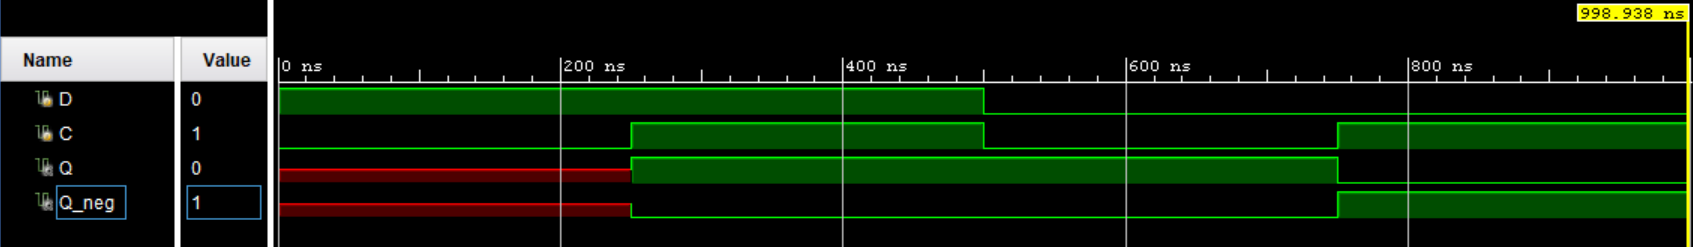
\includegraphics[width=1\textwidth]{tests/test-D Latch.png}
	\caption{D Latch Simulation}
	\label{fig7}
\end{figure}
\begin{center}
\[Q^+ = D\]
It is clear from simulation that D input determines the subsequent state. The D latch equation is therefore Q(t+1) = D.
\end{center}

\subsection{Part 4}
\parts{JK Flip Flop}

\subsection{Part 5}
\parts{Asynchronous Up Counter}
\begin{center}
\begin{tabular}{c | c c c c }
Count & $Q_3$(MSB) & $Q_2$ & $Q_1$ & $Q_0$(LSB) \\
\hline 
0 & 0 & 0 & 0 & 0 \\
1 & 0 & 0 & 0 & 1 \\
2 & 0 & 0 & 1 & 0 \\
3 & 0 & 0 & 1 & 1 \\
4 & 0 & 1 & 0 & 0 \\
5 & 0 & 1 & 0 & 1 \\
6 & 0 & 1 & 1 & 0 \\
7 & 0 & 1 & 1 & 1 \\
8 & 1 & 0 & 0 & 0 \\
9 & 1 & 0 & 0 & 1 \\
10 & 1 & 0 & 1 & 0 \\
11 & 1 & 0 & 1 & 1 \\
12 & 1 & 1 & 0 & 0 \\
13 & 1 & 1 & 0 & 1 \\
14 & 1 & 1 & 1 & 0 \\
15 & 1 & 1 & 1 & 1 \\
0 & 0 & 0 & 0 & 0 \\
\end{tabular}\par\vspace{1em}
 Truth Table of Asynchronous Up Counter
\end{center}
%%%%%%%%%%%%%%%%%%%%%%%%%%%%%%%%%%%%%%%%%%%%%%%%%%%%%%%%%%%%%%%%%%%%%%%%%%%%%%%%%%%%%%%%%%%%%%%%%%%%
\subsection{Part 6}
\parts{Synchronous Up Counter}
\begin{center}
\begin{tabular}{c | c c c c }
Count & $Q_3$(MSB) & $Q_2$ & $Q_1$ & $Q_0$(LSB) \\
\hline 
0 & 0 & 0 & 0 & 0 \\
1 & 0 & 0 & 0 & 1 \\
2 & 0 & 0 & 1 & 0 \\
3 & 0 & 0 & 1 & 1 \\
4 & 0 & 1 & 0 & 0 \\
5 & 0 & 1 & 0 & 1 \\
6 & 0 & 1 & 1 & 0 \\
7 & 0 & 1 & 1 & 1 \\
8 & 1 & 0 & 0 & 0 \\
9 & 1 & 0 & 0 & 1 \\
10 & 1 & 0 & 1 & 0 \\
11 & 1 & 0 & 1 & 1 \\
12 & 1 & 1 & 0 & 0 \\
13 & 1 & 1 & 0 & 1 \\
14 & 1 & 1 & 1 & 0 \\
15 & 1 & 1 & 1 & 1 \\
0 & 0 & 0 & 0 & 0 \\
\end{tabular}\par\vspace{1em}
 Truth Table of Synchronous Up Counter
\end{center}

\subsection{Part 7}
\begin{figure}[H]
	\centering
	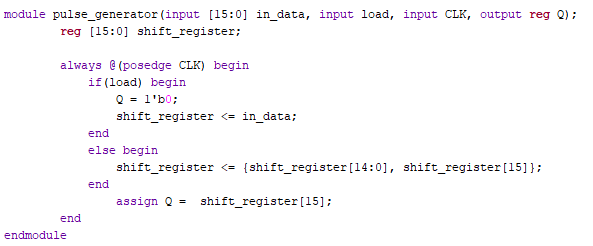
\includegraphics[width=1\textwidth]{codes/code-Pulse Generator.png}
	\caption{Pulse Generator Code}
	\label{fig7}
    \end{figure}
\begin{figure}[H]
	\centering
	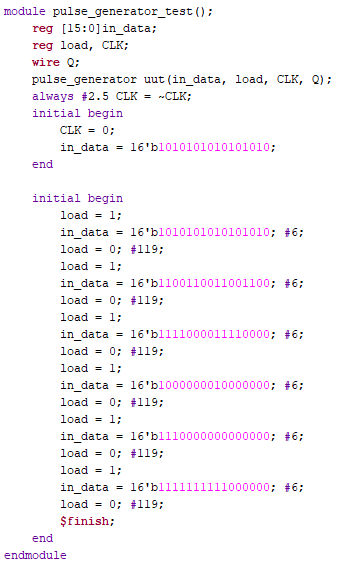
\includegraphics[width=1\textwidth]{codes/code-Pulse Generator Sim.png}
	\caption{Pulse Generator Simulation Code}
	\label{fig7}
    \end{figure}
\begin{figure}[H]
	\centering
	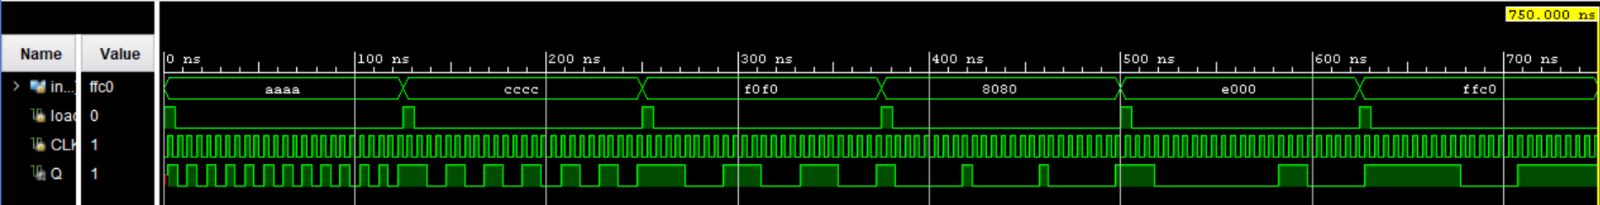
\includegraphics[width=1\textwidth]{tests/test-Pulse Generator.png}
	\caption{Pulse Generator Simulation}
	\label{fig7}
\end{figure}

\begin{center}
The provided 16-bit input value is loaded when the load input is 1, along with the clock signal. The output is the most significant bit of the loaded value. And circular shift operation is completed when the load input is 1, along with the clock signal.
\end{center}

\section{RESULTS}
Every circuit in the homework assignment is implemented using Verilog. The test results supported what we had predicted based on our calculations on paper. All test results are given on the relevant section.

\section{DISCUSSION}
With the help of the verilog programming language, we learned how to implement and use various latches and flip flops through this homework. Using the clock signal, we also learned how to simulate these circuits. Additionally, we learned how to implement frequency design and create synchronous and asynchronous counters. Our outcomes were fully in line with what we had anticipated.

\section{CONCLUSION}
With the help of the verilog programming language, we were able to simulate flip-flops, latches and  counters and learned how to implement them through this homework. To sum up, this was a rather lengthy and challenging homework assignment for us, but we were able to successfully complete all of the parts.

\newpage
\end{document}